\documentclass[]{article}

\usepackage[pdftex]{graphicx}
\usepackage[top=1in, bottom=1in, right=1.25in, left=1.25in]{geometry}
\usepackage{hyperref}

\begin{document}

	\setlength{\parindent}{0pt}
	\setlength{\parskip}{6pt}

	% Title Page
	\begin{titlepage}



		\title{\textbf{ProPANE User Guide}}
		\author{BU ProPANE Team:\\Griffin Dunn\\Colin Madigan\\Phillip Stahlfeld}
		\date{April 28, 2013}
		\maketitle

\begin{figure}[h]
\centering
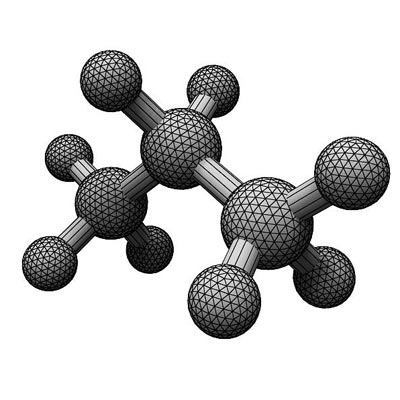
\includegraphics[scale=0.3]{images/logo}
\end{figure}

		\noindent
		
		This is the User's Guide for the ProPANE system.  It teaches the user all necessary information on how to use the ProPANE app and interface with the analysis system.  It also provides helpful suggestions to get the most out of an image capture session. 
		\thispagestyle{empty}
		
		
		
	\end{titlepage}
	
	
	
	
	% Begin  Real  Document
	\pagenumbering{roman}
	\tableofcontents
	\newpage
	
	\pagenumbering{arabic}
	\setcounter{page}{1}
	\thispagestyle{empty}
	
	\section{Capturing a Lecture with ProPANE}
		This section explains how to use the Samsung Galaxy Camera and the ProPANE app to capture a lecture.
		
		\subsection{Positioning the Tripod}
			The ProPANE system currently supports the capture of images from a single whiteboard.  The camera and tripod should be placed so the camera points straight at the desired board. The app supports optical zoom at a high enough resolution as to capture high-quality images from any distance from the board that can be achieved in a classroom. To set up the camera on the tripod, follow these steps:
			\begin{enumerate}
			\item{Extend both sections of each leg of the tripod by unclamping each clamp, sliding the leg to the desired length, and reclamping.}
			\item{Spread the legs of the tripod so it can stand freely.}
			\item{To raise the head of the tripod, unscrew the locking knob at the base of the neck, which holds the neck in place.  Rotate the crank to raise the neck to the desired height, then re-lock the knob.}
			\item{To attach the camera, remove the top piece from the head of the tripod and screw it on to the bottom of the camera, then clip back on to the tripod.}
			\item{The handle attached to the head of the tripod controls the vertical rotation of the tripod head.  Turn the handle to lock or unlock rotation.}
			\end{enumerate} 
		
\begin{figure}[h]
\centering
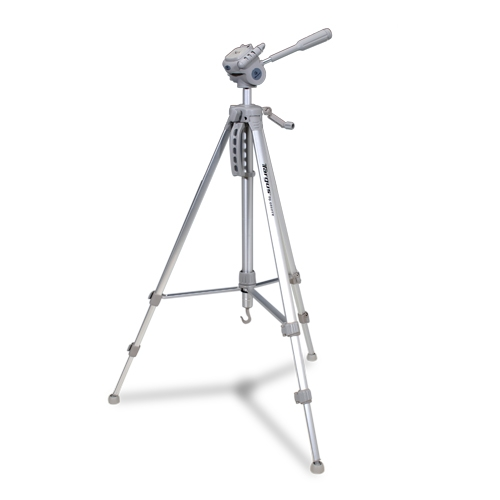
\includegraphics[scale=0.3]{images/tripod}
\caption{The tripod used with the ProPANE system.}
\end{figure}	
			
		\subsection{Starting a Capture}
			After the camera is securely attached to the tripod, start the ProPANE app.  Turn on the Samsung Galaxy Camera by holding the power button for a moment.  A shortcut to the ProPANE app should be on the home screen that greets you on start-up.  If the shortcut is not visible, press ``Apps'' and browse until you find the ProPANE app.  Use the button in the app to set the resolution of images during the capture set.  Next, use the preview image on the screen to point the camera at the board.  Make sure the entire desired capture area is visible in the preview image.  If necessary, zoom in or out using the in-app buttons.  If the image does not look focused, don't worry --- it will become focused after starting the capture.  When everything is set as desired, hit the ``Start Capture'' button. \\ \\

\textbf{Note:} Make sure that upon hitting ``Start Capture'', the view of the whiteboard is unimpeded.  The analysis will not work correctly unless the first captured image contains the empty whiteboard. \\ \\			
			 When all desired images have been captured, hit the ``Stop Capture'' button.  The screen will shut off during capture.  This is normal.  To turn it back on, press (do not hold) the power button.
			
\begin{figure}[h]
\centering
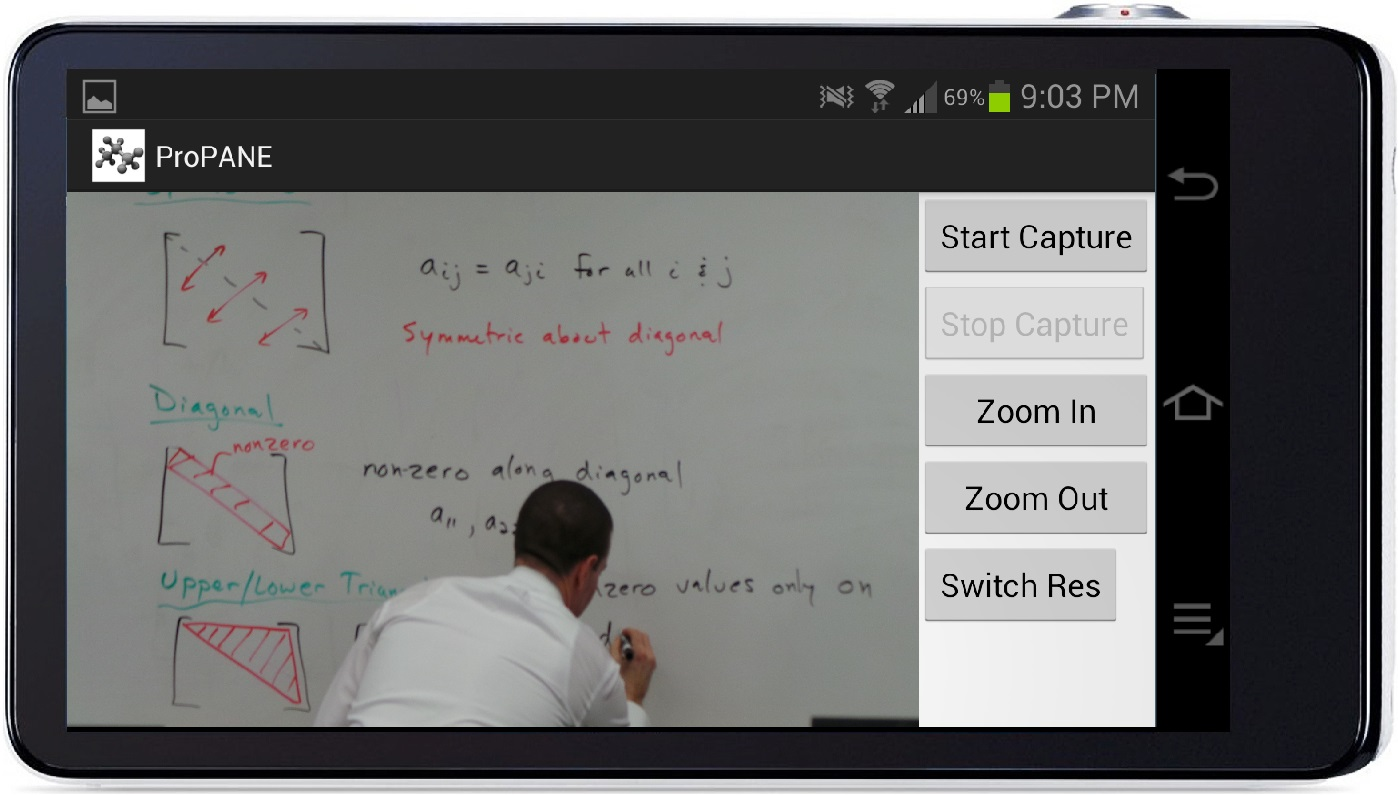
\includegraphics[scale=0.15]{images/app}
\caption{The ProPANE app running on the Samsung Galaxy Camera.}
\end{figure}
		\section{Interacting with the analysis system}
		The Galaxy Camera provides the user with multiple ways to upload image sets to the ProPANE analysis system.  
		\subsection{Uploading images via Wi-Fi}
		Images can be wirelessly uploaded using the free AndSMB app, which has been installed on the Galaxy Camera. To do this:
	
		\begin{enumerate}
		\item{Make sure the camera is connected to the bucknell.edu wireless network.}
		\item{Open the AndSMB app from the ``Apps'' screen}
		\item{Under ``Select your SMB Server:'' press the ``Add'' button.}
		\item{Next to ``Hostname'' type: $propane.stahlfeld.com$}
		\item{Next to both ``Username'' and ``Password'' type: $propane$}
		\item{A list of folders will appear.  Press the folder named ``ProPane'', followed by the folder named ``new\_ captures''}
		\item{At the top left of the screen, press ``Device file browser''}
		\item{Using the on-screen buttons, navigate to the directory $/storage/sdcard0/Pictures/ProPANE$}
		\item{Each folder in this directory contains a different capture set.  The time of capture is listed on the right.  Select the desired capture set by holding your finger on the folder until a green check mark appears over the folder icon.}
		\item{Press the ``Upload'' button at the top center of the screen, and then press ``Ok''}
		\end{enumerate}

The selected images will be uploaded to the ProPANE server, and can be retrieved from any computer file browser.
		\subsection{Uploading images via USB with a Windows computer}
		The images can also be uploaded by plugging the camera into a computer running Windows and uploading to the ProPANE server.  To do this:
		\begin{enumerate}
		\item{Make sure the computer is connected to the bucknell.edu network.}
		\item{Using the provided USB-to-Micro-USB cable, connect the camera to the computer.  Make sure the camera is turned on first.}
		\item{Using Windows Explorer, navigate to ``Computer'', then double-click on the icon labeled ``SAMSUNG -EK-GC100'' under the ``Portable Devices'' section.}
		\item{Navigate to the directory \textit{Camera\textbackslash Pictures\textbackslash ProPANE}.  All capture set folders are located here.  The folders are named using a timestamp indicating when they were created, so use this to determine which folder is the desired capture set.}
		\item{Open a second Windows Explorer window.  In the address bar, type $\\propane.stahlfeld.com$}
		\item{Double-click on the ``ProPane'' folder.  When prompted for a username and password, type $propane$ for both.}
		\item{Drag the desired image set folder from the camera file directory to the folder called ``new\_captures'' on the ProPANE server.}
		\end{enumerate}
		
		The selected images will be uploaded to the ProPANE server, and can be retrieved from any computer file browser. \\ \\
		\textbf{Note:} These instructions detail the process for Windows 7, but it should be very similar for previous versions of Windows.
		
		\subsection{Viewing key images}	
		After the analysis process has finished, your images will be available in a folder named ``out'' which is created in the original image folder that was uploaded to ``new\_captures''.  This folder is still located in ``new\_captures''.  The key images are the images with names containing the phrase $keyimg$.  These can be dragged and saved in any folder on your local computer.  Also present are a series of debug images, helpful for seeing the progression of the capture.  In the unlikely event that important information is missed by all key images, it can be found in the debug images.  
		
		
		\section{Helpful Information}
		The ProPANE system is robust and flexible, but to optimize the results, it is recommended that users follow these guidelines when capturing information.
		
		\begin{itemize}
		\item{Make sure that upon hitting ``Start Capture'', the view of the whiteboard is unimpeded.  The analysis will not work correctly unless the first captured image contains the empty whiteboard. }
		\item{Try to stand out from the color of the board.  Wear a dark shirt, ideally with long sleeves.  White shirts appear very similar to the board in the eye of the camera, and skin reflects light in a similar manner.  Shirts with stripes that greatly contrast the main shirt color, or feature text, may also decrease the accuracy of results.}
		\item{The analysis system is optimized for the capture of information on one whiteboard.  If you are trying to capture more than one board, the results cannot be guaranteed. }
		\item{During a capture session, keep the lighting in the room as constant as possible.  Highly lit rooms produce the best results.}
		
		\end{itemize}
		
\end{document}